% Options for packages loaded elsewhere
\PassOptionsToPackage{unicode}{hyperref}
\PassOptionsToPackage{hyphens}{url}
\PassOptionsToPackage{dvipsnames,svgnames*,x11names*}{xcolor}
%
\documentclass[
  ignorenonframetext,
  UTF8,fontset=adobe,zihao=false]{ctexbeamer}
\usepackage{pgfpages}
\setbeamertemplate{caption}[numbered]
\setbeamertemplate{caption label separator}{: }
\setbeamercolor{caption name}{fg=normal text.fg}
\beamertemplatenavigationsymbolsempty
% Prevent slide breaks in the middle of a paragraph
\widowpenalties 1 10000
\raggedbottom
\usepackage{lmodern}
\usepackage{amssymb,amsmath}
\usepackage{ifxetex,ifluatex}
\ifnum 0\ifxetex 1\fi\ifluatex 1\fi=0 % if pdftex
  \usepackage[T1]{fontenc}
  \usepackage[utf8]{inputenc}
  \usepackage{textcomp} % provide euro and other symbols
\else % if luatex or xetex
  \usepackage{unicode-math}
  \defaultfontfeatures{Scale=MatchLowercase}
  \defaultfontfeatures[\rmfamily]{Ligatures=TeX,Scale=1}
\fi
\usetheme[colorblocks,showheader,red]{Verona}
% Use upquote if available, for straight quotes in verbatim environments
\IfFileExists{upquote.sty}{\usepackage{upquote}}{}
\IfFileExists{microtype.sty}{% use microtype if available
  \usepackage[]{microtype}
  \UseMicrotypeSet[protrusion]{basicmath} % disable protrusion for tt fonts
}{}
\makeatletter
\@ifundefined{KOMAClassName}{% if non-KOMA class
  \IfFileExists{parskip.sty}{%
    \usepackage{parskip}
  }{% else
    \setlength{\parindent}{0pt}
    \setlength{\parskip}{6pt plus 2pt minus 1pt}}
}{% if KOMA class
  \KOMAoptions{parskip=half}}
\makeatother
\usepackage{xcolor}
\IfFileExists{xurl.sty}{\usepackage{xurl}}{} % add URL line breaks if available
\IfFileExists{bookmark.sty}{\usepackage{bookmark}}{\usepackage{hyperref}}
\hypersetup{
  pdftitle={R Markdown 制作 beamer 幻灯片},
  pdfauthor={黄湘云},
  colorlinks=true,
  linkcolor=Maroon,
  filecolor=Maroon,
  citecolor=Blue,
  urlcolor=Blue,
  pdfcreator={LaTeX via pandoc}}
\urlstyle{same} % disable monospaced font for URLs
\newif\ifbibliography
\usepackage{color}
\usepackage{fancyvrb}
\newcommand{\VerbBar}{|}
\newcommand{\VERB}{\Verb[commandchars=\\\{\}]}
\DefineVerbatimEnvironment{Highlighting}{Verbatim}{commandchars=\\\{\}}
% Add ',fontsize=\small' for more characters per line
\usepackage{framed}
\definecolor{shadecolor}{RGB}{248,248,248}
\newenvironment{Shaded}{\begin{snugshade}}{\end{snugshade}}
\newcommand{\AlertTok}[1]{\textcolor[rgb]{0.94,0.16,0.16}{#1}}
\newcommand{\AnnotationTok}[1]{\textcolor[rgb]{0.56,0.35,0.01}{\textbf{\textit{#1}}}}
\newcommand{\AttributeTok}[1]{\textcolor[rgb]{0.77,0.63,0.00}{#1}}
\newcommand{\BaseNTok}[1]{\textcolor[rgb]{0.00,0.00,0.81}{#1}}
\newcommand{\BuiltInTok}[1]{#1}
\newcommand{\CharTok}[1]{\textcolor[rgb]{0.31,0.60,0.02}{#1}}
\newcommand{\CommentTok}[1]{\textcolor[rgb]{0.56,0.35,0.01}{\textit{#1}}}
\newcommand{\CommentVarTok}[1]{\textcolor[rgb]{0.56,0.35,0.01}{\textbf{\textit{#1}}}}
\newcommand{\ConstantTok}[1]{\textcolor[rgb]{0.00,0.00,0.00}{#1}}
\newcommand{\ControlFlowTok}[1]{\textcolor[rgb]{0.13,0.29,0.53}{\textbf{#1}}}
\newcommand{\DataTypeTok}[1]{\textcolor[rgb]{0.13,0.29,0.53}{#1}}
\newcommand{\DecValTok}[1]{\textcolor[rgb]{0.00,0.00,0.81}{#1}}
\newcommand{\DocumentationTok}[1]{\textcolor[rgb]{0.56,0.35,0.01}{\textbf{\textit{#1}}}}
\newcommand{\ErrorTok}[1]{\textcolor[rgb]{0.64,0.00,0.00}{\textbf{#1}}}
\newcommand{\ExtensionTok}[1]{#1}
\newcommand{\FloatTok}[1]{\textcolor[rgb]{0.00,0.00,0.81}{#1}}
\newcommand{\FunctionTok}[1]{\textcolor[rgb]{0.00,0.00,0.00}{#1}}
\newcommand{\ImportTok}[1]{#1}
\newcommand{\InformationTok}[1]{\textcolor[rgb]{0.56,0.35,0.01}{\textbf{\textit{#1}}}}
\newcommand{\KeywordTok}[1]{\textcolor[rgb]{0.13,0.29,0.53}{\textbf{#1}}}
\newcommand{\NormalTok}[1]{#1}
\newcommand{\OperatorTok}[1]{\textcolor[rgb]{0.81,0.36,0.00}{\textbf{#1}}}
\newcommand{\OtherTok}[1]{\textcolor[rgb]{0.56,0.35,0.01}{#1}}
\newcommand{\PreprocessorTok}[1]{\textcolor[rgb]{0.56,0.35,0.01}{\textit{#1}}}
\newcommand{\RegionMarkerTok}[1]{#1}
\newcommand{\SpecialCharTok}[1]{\textcolor[rgb]{0.00,0.00,0.00}{#1}}
\newcommand{\SpecialStringTok}[1]{\textcolor[rgb]{0.31,0.60,0.02}{#1}}
\newcommand{\StringTok}[1]{\textcolor[rgb]{0.31,0.60,0.02}{#1}}
\newcommand{\VariableTok}[1]{\textcolor[rgb]{0.00,0.00,0.00}{#1}}
\newcommand{\VerbatimStringTok}[1]{\textcolor[rgb]{0.31,0.60,0.02}{#1}}
\newcommand{\WarningTok}[1]{\textcolor[rgb]{0.56,0.35,0.01}{\textbf{\textit{#1}}}}
\usepackage{longtable,booktabs}
\usepackage{caption}
% Make caption package work with longtable
\makeatletter
\def\fnum@table{\tablename~\thetable}
\makeatother
\usepackage{graphicx,grffile}
\makeatletter
\def\maxwidth{\ifdim\Gin@nat@width>\linewidth\linewidth\else\Gin@nat@width\fi}
\def\maxheight{\ifdim\Gin@nat@height>\textheight\textheight\else\Gin@nat@height\fi}
\makeatother
% Scale images if necessary, so that they will not overflow the page
% margins by default, and it is still possible to overwrite the defaults
% using explicit options in \includegraphics[width, height, ...]{}
\setkeys{Gin}{width=\maxwidth,height=\maxheight,keepaspectratio}
% Set default figure placement to htbp
\makeatletter
\def\fps@figure{htbp}
\makeatother
\usepackage[normalem]{ulem}
% Avoid problems with \sout in headers with hyperref
\pdfstringdefDisableCommands{\renewcommand{\sout}{}}
\setlength{\emergencystretch}{3em} % prevent overfull lines
\providecommand{\tightlist}{%
  \setlength{\itemsep}{0pt}\setlength{\parskip}{0pt}}
\setcounter{secnumdepth}{5}
\logo{\includegraphics[height=0.8cm]{C:/PROGRA~1/R/R-40~1.0/doc/html/Rlogo}}
\usepackage[]{natbib}
\bibliographystyle{apalike}

\title{R Markdown 制作 beamer 幻灯片}
\author{黄湘云}
\date{2020-06-13}
\institute{中国矿业大学(北京)}

\begin{document}
\frame{\titlepage}

\hypertarget{intro}{%
\section{介绍}\label{intro}}

\begin{frame}{目录}
\protect\hypertarget{outline}{}

\begin{enumerate}
\item
  Markdown

  \begin{enumerate}
  \tightlist
  \item
    John Gruber's Markdown
  \item
    Pandoc's Markdown
  \item
    Hugo's Markdown/Blackfriday's Markdown
  \item
    R Markdown
  \end{enumerate}
\item
  R Markdown

  \begin{enumerate}
  \tightlist
  \item
    Pandoc
  \item
    LaTeX
  \item
    CSS/JS/HTML
  \item
    Lua
  \end{enumerate}
\item
  Pandoc

  \begin{enumerate}
  \tightlist
  \item
    Haskell
  \end{enumerate}
\end{enumerate}

\end{frame}

\begin{frame}{R 语言}
\protect\hypertarget{sec:rlang}{}

\begin{quotation}[John Gruber]

A Markdown-formatted document should be publishable as-is, as plain text,
without looking like it's been marked up with tags or formatting instructions.

\end{quotation}

Markdown 提供一种简洁的格式语法,用来编辑 HTML、PDF 和 MS Word 文档。
介绍 R Markodwn 文档如何插入图片,更多详情见 \url{https://rmarkdown.rstudio.com} \citep{rmarkdown2018}。

R 语言的命名部分来源于最初的两位作者的姓名的首字母 Robert Gentleman 和 Ross Ihaka,
部分是由于贝尔实验室推出的 S 语言 \citep{base}。

\end{frame}

\begin{frame}{Markdown 语法}
\protect\hypertarget{sec:markdown}{}

\begin{description}
\tightlist
\item[轻微强调]
这是倾斜的文字 \emph{下划线表示强调}, and this is \emph{星花表示强调}.
\item[特别强调]
这是加粗的文字 \textbf{strong emphasis} and \textbf{with underscores}.
\item[强烈强调]
这是斜体加粗的文字 \textbf{\emph{三个星花}}
\item[删除线]
This \sout{is deleted text.}
\item[上下标]
H\textsubscript{2}O is a liquid. 2\textsuperscript{10} is 1024. C\textsuperscript{137} 是一种放射性元素
\end{description}

\begin{longtable}[]{@{}ll@{}}
\caption[\label{tab:insert-tab} 表格标题]{\label{tab:insert-tab} 表格标题\footnote<.->{附有脚注}}\tabularnewline
\toprule
First Header & Second Header\tabularnewline
\midrule
\endfirsthead
\toprule
First Header & Second Header\tabularnewline
\midrule
\endhead
Content Cell & Content Cell\tabularnewline
Content Cell & Content Cell\tabularnewline
\bottomrule
\end{longtable}

\end{frame}

\begin{frame}[fragile]{Markdown 插图}
\protect\hypertarget{sec:fig-markdown}{}

中括号、小括号、大括号分别对应图片标题、路径、属性

\begin{Shaded}
\begin{Highlighting}[]
\AlertTok{![...](...)}\NormalTok{\{...\}}
\end{Highlighting}
\end{Shaded}

\begin{figure}
\centering
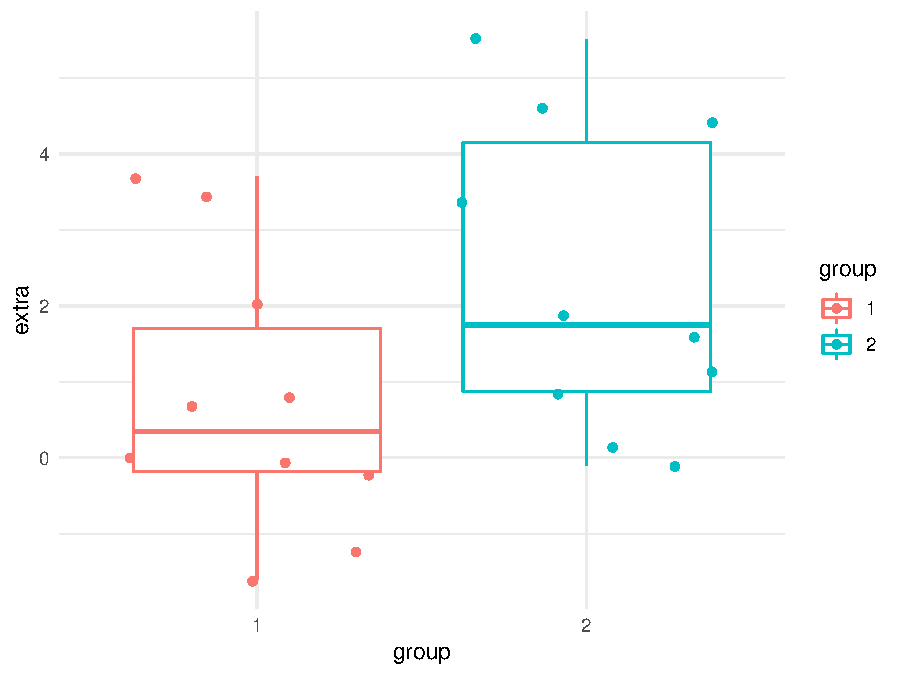
\includegraphics[width=0.5\textwidth,height=\textheight]{beamer-verona_files/figure-beamer/sleep-1.pdf}
\caption[\label{fig:fig-markdown} 默认图片位置居左]{\label{fig:fig-markdown} 默认图片位置居左\footnotemark{}}
\end{figure}
\footnotetext{这里是脚注}

\end{frame}

\begin{frame}{睡眠数据 sleep}
\protect\hypertarget{sec:sleep}{}

\begin{figure}
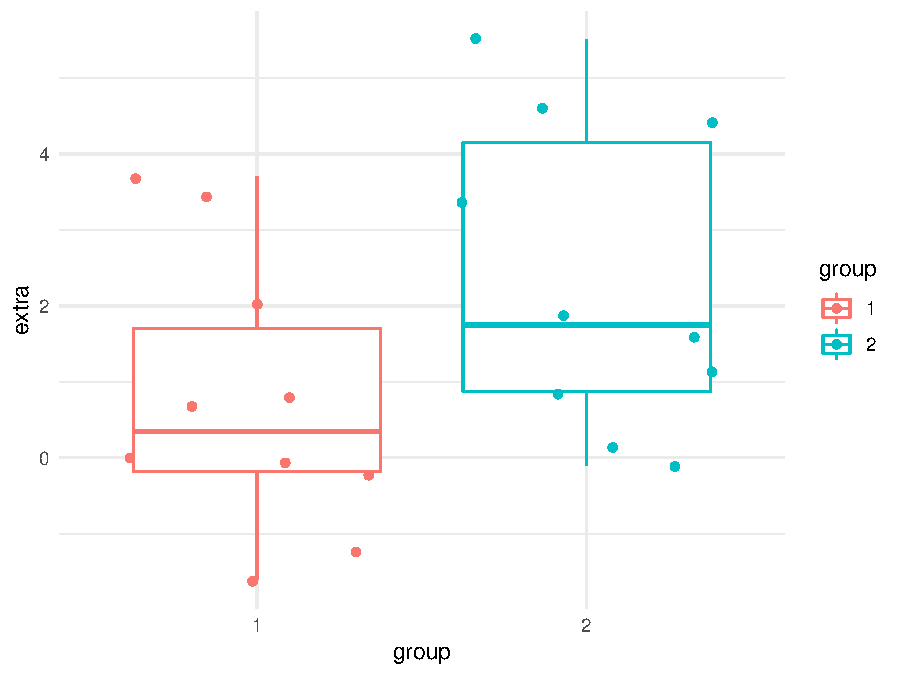
\includegraphics[width=0.7\linewidth]{beamer-verona_files/figure-beamer/sleep-1} \caption{药物对睡眠时长的影响}\label{fig:sleep}
\end{figure}

\end{frame}

\begin{frame}{压力数据 pressure}
\protect\hypertarget{sec:pressure}{}

\begin{figure}
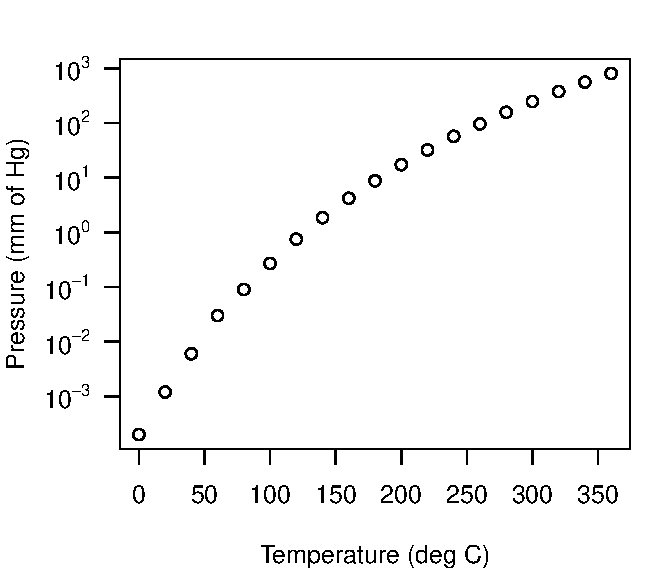
\includegraphics[width=0.65\linewidth]{beamer-verona_files/figure-beamer/pressure-1} \caption{压力和温度的关系}\label{fig:pressure}
\end{figure}

\end{frame}

\begin{frame}[fragile]{设置主题}
\protect\hypertarget{sec:setup-verona}{}

Ivan Valbusa 开发了 \href{https://bitbucket.org/rivanvx/beamer}{Verona 主题的 Beamer 模版},
目前 CTAN 上的版本是 0.2,文档说明见 \url{https://www.ctan.org/pkg/beamer-verona}
这个主题的宏包依赖很少!我很喜欢!

\begin{Shaded}
\begin{Highlighting}[]
\NormalTok{tinytex}\OperatorTok{::}\KeywordTok{tlmgr_install}\NormalTok{(}\StringTok{'beamer-verona'}\NormalTok{)}
\end{Highlighting}
\end{Shaded}

\end{frame}

\begin{frame}{自定义的块}
\protect\hypertarget{sec:custom-blocks}{}

\begin{quotation}[Donald E. Knuth, The \TeX book]

Gentle reader: This is a handbook about TEX, a new typesetting
system G intended for the creation of beautiful books---and
especially for books that contain a lot of mathematics.

\end{quotation}

\begin{exampleblock}{提示}

提示

\end{exampleblock}

\pause

\begin{alertblock}{警告}

警告

\end{alertblock}

\pause

\begin{block}{注意}

请读者注意

\end{block}

\end{frame}

\begin{frame}[fragile,allowframebreaks]{运行环境}
\protect\hypertarget{session-info}{}

制作此幻灯片,我们使用了 bookdown 包 \citep{bookdown2016}、 rmarkdown 包 \citep{rmarkdown2018} 和 knitr 包 \citep{knitr2015},以及 R version 4.0.0 (2020-04-24) 其它软件和环境信息见下方

\begin{Shaded}
\begin{Highlighting}[]
\NormalTok{xfun}\OperatorTok{::}\KeywordTok{session_info}\NormalTok{(}\KeywordTok{c}\NormalTok{(}
  \StringTok{"bookdown"}\NormalTok{, }\StringTok{"rmarkdown"}\NormalTok{, }\StringTok{"knitr"}
\NormalTok{), }\DataTypeTok{dependencies =} \OtherTok{TRUE}\NormalTok{)}
\end{Highlighting}
\end{Shaded}

\begin{verbatim}
R version 4.0.0 (2020-04-24)
Platform: x86_64-w64-mingw32/x64 (64-bit)
Running under: Windows 10 x64 (build 16299)

Locale:
  LC_COLLATE=Chinese (Simplified)_China.936 
  LC_CTYPE=Chinese (Simplified)_China.936   
  LC_MONETARY=Chinese (Simplified)_China.936
  LC_NUMERIC=C                              
  LC_TIME=Chinese (Simplified)_China.936    

Package version:
  base64enc_0.1.3 bookdown_0.19   digest_0.6.25   evaluate_0.14  
  glue_1.4.1      graphics_4.0.0  grDevices_4.0.0 highr_0.8      
  htmltools_0.4.0 jsonlite_1.6.1  knitr_1.28      magrittr_1.5   
  markdown_1.1    methods_4.0.0   mime_0.9        Rcpp_1.0.4.6   
  rlang_0.4.6     rmarkdown_2.2   stats_4.0.0     stringi_1.4.6  
  stringr_1.4.0   tinytex_0.23    tools_4.0.0     utils_4.0.0    
  xfun_0.14       yaml_2.2.1     

Pandoc version: 2.7.3
\end{verbatim}

\end{frame}

\renewcommand\refname{参考文献}
\begin{frame}[allowframebreaks]{参考文献}
  \bibliographytrue
  \bibliography{packages.bib}
\end{frame}

\end{document}
